\documentclass{standalone}
\usepackage{tikz}
\usepackage{ctex,siunitx}
\setCJKmainfont{Noto Serif CJK SC}
\usepackage{tkz-euclide}
\usepackage{amsmath}
\usepackage{wasysym}
\usetikzlibrary{patterns, calc}
\usetikzlibrary {decorations.pathmorphing, decorations.pathreplacing, decorations.shapes,}
\begin{document}
\small
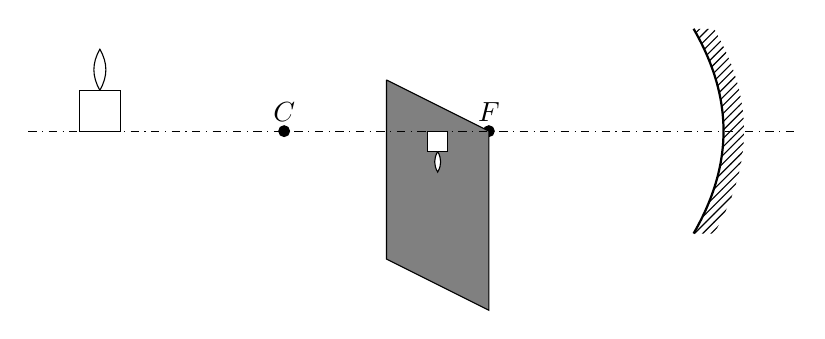
\begin{tikzpicture}[>=latex,scale=1.3]
  \fill [pattern=north east lines] (2,-1)--(2.2,-1) to [bend left=-30] (2.2,1) --(2,1) to [bend left=30](2,-1);
  \draw [thick](2,1) to [bend left=30] (2,-1);
  \node at (0,0)[above]{$F$}; \draw [fill=black] (0,0) circle(1.5pt);
  \node at (-2,0)[above]{$C$}; \draw [fill=black] (-2,0) circle(1.5pt);
  \draw (-4,0) rectangle (-3.6,.4); \draw (-3.8, .4) to [bend left=-30](-3.8, .8)to [bend left=-30] (-3.8,.4) ;
  \draw [fill=gray] (-1, .5)--(-1,-1.25)--(0, -1.75)--(0, 0)--(-1, .5);
  \draw [fill=white](-.5-.1,0) rectangle (-.5+.1,-.2); \draw [fill=white] (-.5, -.2) to [bend left=-30](-.5, -.4)to [bend left=-30] (-.5, -.2) ;
  \draw[dashdotted] (-4.5,0)--(3,0);
\end{tikzpicture}
\end{document}